% Options for packages loaded elsewhere
\PassOptionsToPackage{unicode}{hyperref}
\PassOptionsToPackage{hyphens}{url}
%
\documentclass[
]{article}
\usepackage{amsmath,amssymb}
\usepackage{lmodern}
\usepackage{iftex}
\ifPDFTeX
  \usepackage[T1]{fontenc}
  \usepackage[utf8]{inputenc}
  \usepackage{textcomp} % provide euro and other symbols
\else % if luatex or xetex
  \usepackage{unicode-math}
  \defaultfontfeatures{Scale=MatchLowercase}
  \defaultfontfeatures[\rmfamily]{Ligatures=TeX,Scale=1}
\fi
% Use upquote if available, for straight quotes in verbatim environments
\IfFileExists{upquote.sty}{\usepackage{upquote}}{}
\IfFileExists{microtype.sty}{% use microtype if available
  \usepackage[]{microtype}
  \UseMicrotypeSet[protrusion]{basicmath} % disable protrusion for tt fonts
}{}
\makeatletter
\@ifundefined{KOMAClassName}{% if non-KOMA class
  \IfFileExists{parskip.sty}{%
    \usepackage{parskip}
  }{% else
    \setlength{\parindent}{0pt}
    \setlength{\parskip}{6pt plus 2pt minus 1pt}}
}{% if KOMA class
  \KOMAoptions{parskip=half}}
\makeatother
\usepackage{xcolor}
\usepackage{color}
\usepackage{fancyvrb}
\newcommand{\VerbBar}{|}
\newcommand{\VERB}{\Verb[commandchars=\\\{\}]}
\DefineVerbatimEnvironment{Highlighting}{Verbatim}{commandchars=\\\{\}}
% Add ',fontsize=\small' for more characters per line
\newenvironment{Shaded}{}{}
\newcommand{\AlertTok}[1]{\textcolor[rgb]{1.00,0.00,0.00}{\textbf{#1}}}
\newcommand{\AnnotationTok}[1]{\textcolor[rgb]{0.38,0.63,0.69}{\textbf{\textit{#1}}}}
\newcommand{\AttributeTok}[1]{\textcolor[rgb]{0.49,0.56,0.16}{#1}}
\newcommand{\BaseNTok}[1]{\textcolor[rgb]{0.25,0.63,0.44}{#1}}
\newcommand{\BuiltInTok}[1]{\textcolor[rgb]{0.00,0.50,0.00}{#1}}
\newcommand{\CharTok}[1]{\textcolor[rgb]{0.25,0.44,0.63}{#1}}
\newcommand{\CommentTok}[1]{\textcolor[rgb]{0.38,0.63,0.69}{\textit{#1}}}
\newcommand{\CommentVarTok}[1]{\textcolor[rgb]{0.38,0.63,0.69}{\textbf{\textit{#1}}}}
\newcommand{\ConstantTok}[1]{\textcolor[rgb]{0.53,0.00,0.00}{#1}}
\newcommand{\ControlFlowTok}[1]{\textcolor[rgb]{0.00,0.44,0.13}{\textbf{#1}}}
\newcommand{\DataTypeTok}[1]{\textcolor[rgb]{0.56,0.13,0.00}{#1}}
\newcommand{\DecValTok}[1]{\textcolor[rgb]{0.25,0.63,0.44}{#1}}
\newcommand{\DocumentationTok}[1]{\textcolor[rgb]{0.73,0.13,0.13}{\textit{#1}}}
\newcommand{\ErrorTok}[1]{\textcolor[rgb]{1.00,0.00,0.00}{\textbf{#1}}}
\newcommand{\ExtensionTok}[1]{#1}
\newcommand{\FloatTok}[1]{\textcolor[rgb]{0.25,0.63,0.44}{#1}}
\newcommand{\FunctionTok}[1]{\textcolor[rgb]{0.02,0.16,0.49}{#1}}
\newcommand{\ImportTok}[1]{\textcolor[rgb]{0.00,0.50,0.00}{\textbf{#1}}}
\newcommand{\InformationTok}[1]{\textcolor[rgb]{0.38,0.63,0.69}{\textbf{\textit{#1}}}}
\newcommand{\KeywordTok}[1]{\textcolor[rgb]{0.00,0.44,0.13}{\textbf{#1}}}
\newcommand{\NormalTok}[1]{#1}
\newcommand{\OperatorTok}[1]{\textcolor[rgb]{0.40,0.40,0.40}{#1}}
\newcommand{\OtherTok}[1]{\textcolor[rgb]{0.00,0.44,0.13}{#1}}
\newcommand{\PreprocessorTok}[1]{\textcolor[rgb]{0.74,0.48,0.00}{#1}}
\newcommand{\RegionMarkerTok}[1]{#1}
\newcommand{\SpecialCharTok}[1]{\textcolor[rgb]{0.25,0.44,0.63}{#1}}
\newcommand{\SpecialStringTok}[1]{\textcolor[rgb]{0.73,0.40,0.53}{#1}}
\newcommand{\StringTok}[1]{\textcolor[rgb]{0.25,0.44,0.63}{#1}}
\newcommand{\VariableTok}[1]{\textcolor[rgb]{0.10,0.09,0.49}{#1}}
\newcommand{\VerbatimStringTok}[1]{\textcolor[rgb]{0.25,0.44,0.63}{#1}}
\newcommand{\WarningTok}[1]{\textcolor[rgb]{0.38,0.63,0.69}{\textbf{\textit{#1}}}}
\usepackage{longtable,booktabs,array}
\usepackage{calc} % for calculating minipage widths
% Correct order of tables after \paragraph or \subparagraph
\usepackage{etoolbox}
\makeatletter
\patchcmd\longtable{\par}{\if@noskipsec\mbox{}\fi\par}{}{}
\makeatother
% Allow footnotes in longtable head/foot
\IfFileExists{footnotehyper.sty}{\usepackage{footnotehyper}}{\usepackage{footnote}}
\makesavenoteenv{longtable}
\usepackage{graphicx}
\makeatletter
\def\maxwidth{\ifdim\Gin@nat@width>\linewidth\linewidth\else\Gin@nat@width\fi}
\def\maxheight{\ifdim\Gin@nat@height>\textheight\textheight\else\Gin@nat@height\fi}
\makeatother
% Scale images if necessary, so that they will not overflow the page
% margins by default, and it is still possible to overwrite the defaults
% using explicit options in \includegraphics[width, height, ...]{}
\setkeys{Gin}{width=\maxwidth,height=\maxheight,keepaspectratio}
% Set default figure placement to htbp
\makeatletter
\def\fps@figure{htbp}
\makeatother
\setlength{\emergencystretch}{3em} % prevent overfull lines
\providecommand{\tightlist}{%
  \setlength{\itemsep}{0pt}\setlength{\parskip}{0pt}}
\setcounter{secnumdepth}{-\maxdimen} % remove section numbering
\ifLuaTeX
  \usepackage{selnolig}  % disable illegal ligatures
\fi
\IfFileExists{bookmark.sty}{\usepackage{bookmark}}{\usepackage{hyperref}}
\IfFileExists{xurl.sty}{\usepackage{xurl}}{} % add URL line breaks if available
\urlstyle{same} % disable monospaced font for URLs
\hypersetup{
  hidelinks,
  pdfcreator={LaTeX via pandoc}}

\author{}
\date{}

\begin{document}

\hypertarget{multi-period-compliance-mean-field-game-with-deep-fbsde-solver}{%
\subsection{\# Multi-Period Compliance Mean Field Game with Deep FBSDE
Solver}\label{multi-period-compliance-mean-field-game-with-deep-fbsde-solver}}

This is an research report giving big pictures about the problem we aim
to solve, the key methods/algorithms we propose, the main results we
get, as well as comparisons between different methods and consequent
results.

:bulb: See
\href{../FinalReports/Report-StepwiseDetail.md}{\emph{Report-StepwiseDetail}}
for more math and algorithm details; see \emph{README} files for more
code instructions.

\begin{center}\rule{0.5\linewidth}{0.5pt}\end{center}

\hypertarget{abstract}{%
\subsection{Abstract}\label{abstract}}

The aim of this work is to extend the single-period compliance model in
\href{\%22https://doi.org/10.48550/arXiv.2110.01127\%22}{{[}1{]}} to
multi-period, proposing several tricks to improve the numeric stability
of the deep solver for FBSDEs with jumps. First by reproducing the
aformentioned research by Campbell, Steven, et al.~(2021), then by
considering an additional period to the original model, we make
comparisons between long/short-term perspectives when it comes to
multi-peirod production decision-making in renewable electricity
certificate markets, as well as between different numeric tricks when it
comes to algorithm stability. Meanwhile, some practical takeaways on
parameter-tuning are recorded.

\hypertarget{problem-overview}{%
\subsection{1. Problem Overview}\label{problem-overview}}

Conventional numerical solvers are hard pressed to solve PA-MFG with
market-clearing conditions, which may be faced with the ``curse of
dimentionality'' (Bellman 1957)\footnote{Bellman, R. E.: Dynamic
  Programming. Princeton University Press, USA (1957).}. Thus in their
study \href{\%22https://doi.org/10.48550/arXiv.2110.01127\%22}{{[}1{]}},
Professor Campbell and his fellows proposed an actor-critic approach to
optimization, where the agents form a Nash equilibria according to the
principal's penalty function, and the principal evaluates the resulting
equilibria. And they applies this approach to a stylized PA problem
arising in Renewable Energy Certificate (REC) markets, where agents may
\emph{work} overtime (or \emph{rent} capacity), \emph{trade} RECs, and
\emph{expand} their long-term capacity to navigate the market at maximum
profit. Here we only discuss the agents' problem in the
multi-agent-multi-period scenario.

\hypertarget{rec-market-basics}{%
\subsubsection{1.1. REC Market Basics}\label{rec-market-basics}}

Closely related to carbon cap-and-trade (C\&T) markets, REC markets are
a type of market-based emmissions regulation policies, which are
motivating real-world applications of FBSDEs in modeling PA-MFG.

In RES markets, a regulator plays the role of principle, setting a floor
on the amount of energy generated from renewable resources (aka. green
energy) for each firm (based on a percentage of their total production),
and providing certificates for each MWh of green energy generated and
delivered to the grid. These certificates can be further traded by
individual or companies, i.e.~agents, to: 1) reduce costs or the
greenhouse gas (GHG) emissions impact of their operations; and 2) earn
profits from the extra inventories instead of wasting. Since the
certificates are traded assets, energy suppliers can trade off between
producing clean electricity themselves, and purchasing the certificates
on the market. In all, such policies have played an important role in
funding clean energy development, particularly in past years when the
cost of green power production was not as competitive with the cost of
fossil fuel power.

To ensure compliance, each firm must surrender RECs totaling the floor
at the end of a compliance period, with a monetary penalty paid for each
lacking certificate. And in practice, these systems regulate multiple
consecutive and disjoint compliance periods, which are linked together
through a mechanism called \emph{banking}, where unused allowances in
current period can be carried on to the next period (or multiple future
periods). Thus, as an extension to the single-period framework
\href{\%22https://doi.org/10.48550/arXiv.2110.01127\%22}{{[}1{]}}, we
now consider a 2-period model in this report.\footnote{At a finite set
  of joint points, the posiible lack of differentiability will not have
  any significant affects.}.

\hypertarget{rec-market-modeling-with-fbsdes}{%
\subsubsection{1.2. REC Market Modeling with
FBSDEs}\label{rec-market-modeling-with-fbsdes}}

Let's consider 2 subpopulations here. Before jumping into the 2-period
scenario, we first reproduce the single-period case following steps in
\href{\%22https://doi.org/10.48550/arXiv.2110.01127\%22}{{[}1{]}}. We
denote the period end as \(T\), which can be thought of ``the end of the
world''. Referring to the probabilistic method in
\href{https://arxiv.org/abs/1210.5780}{{[}2{]}} (R. Carmona, F. Delarue,
2012), one can show that, for agent \(i\) in subpopulation \(k\), the
optimal solution to its problem in a \emph{single} period is exactly the
solution to the following coupled FBSDEs:

\[
\begin{aligned}
    &\quad\begin{cases}
        dX_t^{i} &=(h^{k}+g_t^{i}+\Gamma_t^{i}+C_t^{i})dt + \sigma^{k}dW_t^{k}&,  &X_0^{i} \sim \mathcal{N}(v^k,\eta^k)\\
        dC_t^{i} &= a_t^{i}dt &,  &C_0^{i}=0 \\ 
        dY_t^{i} &= Z_t^{k}dW_t^{k}&,  &Y_{T}^{i}=w*\mathbf{1}_{X_{T}^i<K}, \\
    \end{cases} \\
    \\
    &\textit{where}: ~\\
    &\quad\quad\quad Y_t^i := \Bbb{E} \left[w\mathbf{1}_{X_{T}^i< K}|\mathcal{F}_t \right] = w\Bbb{P}\left(X_{T}^i< K ~|~ \mathcal {F}_t\right)\\
    &\quad\quad\quad S_t = \frac{\sum\limits_{k \in \mathcal{k}} {(\frac{\pi^k}{\gamma^k}\mathbb{E}\big[ Y_t^i ~|~ i \in \mathfrak{N}^k; \mathcal{F}_t \big])} }{\sum\limits_{k \in \mathcal{K}}{(\pi^k/\gamma^k)}} \\
    &\quad\quad\quad g_t^k = \frac{Y_t^k}{\zeta^k}\\
    &\quad\quad\quad \Gamma_t^{k} =\frac{Y_t^{k}-S_t}{\gamma^{k}} \\
\end{aligned}
\]

Now consider the 2-agent-2-period MFG with market-clearing conditions.
Let's denote the 2 compliance periods \([0,T_1]\) and \((T_1,T_2]\) as
\(\mathfrak{T_1}\) and \(\mathfrak{T_2}\), respectively. Here we think
of \(T_2\) as ``the end of the world'', after which there are no costs
occurs and all agents forfeit any remaining RECs. Similarly, one can
prove that the optimal operation for agent \(i\) in sub-population
\(k~(\forall~i \in \mathfrak{N}_k,~k\in\lbrace{1,2\rbrace})\) can be
modeled with following coupled FBSDEs:

\[
\begin{cases}
    dX_t^{i} &=(h^{k}+g_t^{i}+\Gamma_t^{i}+C_t^{i})dt + \sigma^{k}dW_t^{k} - \min\left(X_{T_1}^i,K\right)\mathbf{1}_{t=T_1}&,  &X_0^{i} = \zeta^{i} \sim \mathcal{N}(v^k,\eta^k)\\
    dC_t^{i} &= a_t^{i}dt &,  &C_0^{k}=0 \\ 
    dV_t^{i} &= Z_t^{V,k}dW_t^{i}&,  &V_{T_1}^{i}=w*\mathbf{1}_{X^i_{T_1}<K} \\
    dU_t^{i} &= Z_t^{U,k}dW_t^{i}&,  &U_{T_1}^{i}=1*Y_{T_1}^i\mathbf{1}_{X^i_{T_1}>K}\\
    dY_t^{i} &= Z_t^{Y,k}dW_t^{i}&,  &Y_{T_2}^{i}=w*\mathbf{1}_{X^i_{T_2}<K}~~,
\end{cases} \\
~~\\
\begin{aligned}
    \textit{where} &\textit{ the optimal controls are given by:}\\
    & g_t^{i} = \frac{V_t^{i}+U_t^{i}}{\zeta^{k}} ~\mathbf{1}_{t\in [0,T_1]}
                + \frac{Y_t^{i}}{\zeta^{k}} ~\mathbf{1}_{t\in (T_1,T_2]} \\
    & \Gamma_t^{i} =\  \frac{V_t^{i}+U_t^{i}-S_t}{\gamma^{k}} ~\mathbf{1}_{t\in [0,T_1]}
                    + \frac{Y_t^{i}-S_t}{\gamma^{k}} ~\mathbf{1}_{t\in (T_1,T_2]} \\
    & a_t^{i} =\frac{(T_1-t)(V_t^{i}+U_t^{i})+(T_2-T_1)Y^i_t}{\beta^{k}} ~\mathbf{1}_{t\in [0,T_1]}
                + \frac{(T_2-t)Y_t^{i}}{\beta^{k}} ~\mathbf{1}_{t\in (T_1,T_2]} \\
    & S_t = \frac{\sum\limits_{k \in \mathcal{k}} {\frac{\pi^k}{\gamma^k}\mathbb{E}\big[ V_t^i +U_t^i ~|~ i \in \mathfrak{N}^k; \mathcal{F}_t \big]}}{\sum\limits_{k \in \mathcal{K}}{(\pi^k/\gamma^k)}} 
            ~\mathbf{1}_{t\in [0,T_1]} +
            \frac{\sum\limits_{k \in \mathcal{k}} {\frac{\pi^k}{\gamma^k}\mathbb{E}\big[ Y_t^i ~|~ i \in \mathfrak{N}^k; \mathcal{F}_t \big]}}{\sum\limits_{k \in \mathcal{K}}{(\pi^k/\gamma^k)}} 
            ~\mathbf{1}_{t\in (T_1,T_2]} 
\end{aligned}
\]

The key notations/parameters are interpreted as follows:

\begin{itemize}
\item
  \(k \in \mathcal{K}\): a sub-population of agents, within which all
  individuals are assumed to have identical preferences and similar
  initial conditions/capacities, yet across which are distinct. The
  sub-population is annotated by superscript \([\cdot]^{k}\). Here we
  only discuss \(k=1,2\).
\item
  \(i \in \mathfrak{N}\): an individual agent belonging to the
  sub-population \(\mathfrak{N}^k\), annotated by superscript
  \([\cdot]^{i}\).
\item
  \(X_t := (X_t)_{t\in\mathfrak{T_1} \cup \mathfrak{T_2}}\): the current
  inventories in stock. For some key time points:

  \begin{itemize}
  \tightlist
  \item
    at \(t=0\), there may be some stochastics in the initial
    inventories, which are assumed to be normally distributed.
    \(X_0^{i} \sim \mathcal{N}(v^k, \eta^k) ,~ \forall k \in \mathcal{K},~\forall i \in \mathfrak{N}^k\).
  \item
    at \(t=T_1\), the terminal RECs pre-submission are \(X_{T_1}\)
    carried over from the first period. Shortly after forfeiting
    \(\min\Big(K,X^i_{T_1}\Big)\), the remaining inventories in stock
    are \(ReLU\Big(X^i_{T_1}-K\Big)\), which are treated as new initial
    values for the second period.
  \item
    at \(t=T_2\), the terminal RECs pre-submission are \(X^i_{T_2}\).
  \end{itemize}
\item
  \(I_t := (I_t)_{t\in\mathfrak{T_1} \cup \mathfrak{T_2}}\): the
  integrated invetory generation. We introduce this process for
  continuous differentiablity at \(T_1\). And \(X_t\) has the same
  initial conditions as \(I_t\). Clearly, we have:

  \[
    X_t=
    \begin{cases}
        & I_t\quad,                  \quad&& t \in [0,T_1]\\
        & I_t- \min(I_{T_1},K), \quad&& t \in (T_1,T_2]\\
    \end{cases} 
    \quad\text{or}\quad
    X_t=
    \begin{cases}
        & I_t\quad,                                           \quad&& t \in [0,T_1]\\
        & I_t-I_{T_1}+(I_{T_1}-K)_+\quad, \quad&& t \in (T_1,T_2]\\
    \end{cases} 
    \]
\item
  \(K\): the quota that agents must meet at the end of each compliance
  period. Fixed to \(K=0.9\)\footnote{The choice of knot point is
    associated with \(h^{k}\) and total time span \(T_1\), \(T_2\). A
    good target (or quota) should be \textbf{``attainable''} - neither
    too easy nor too hard to achieve. Specifically, even if agents do
    nothing at all, they will have an initial amount plus a baseline
    generation of inventories - for instance, \(0.2*1 + 0.6=0.8\) for
    agents in sub-population 1 at the first period end. Similarly, for
    sub-population 2, all agents will also have a \emph{``garanteed''}
    level of 0.8 for delivery. Thus a target reasonably higher than
    that, i.e.~0.9, would be regard \textbf{``attainable''}.}.
\item
  \(P(\cdot)\): the generic penalty function approximated by
  \emph{\textbf{single-knot penalty functions}} \footnote{See
    \href{../FinalReports/Report-StepwiseDetail.md}{\emph{Report-StepwiseDetail}}
    for more math details.} :
  \[P(x)=w(0.9-x)_+ \Rightarrow\partial_{x}P(x) = - w\mathbf{1}_{x<K}.\]
  Further, by tuning the weight \(w\), we can see the relation between
  the penalty level (controled by \(w\)) and the agents' behaviour, as
  well as its market impact.
\item
  \(h\): the baseline generation rate at which agents generate with zero
  marginal cost.
\item
  \(C_t := (C_t)_{t\in\mathfrak{T_1} \cup \mathfrak{T_2}}\): incremental
  REC capacity of agents, i.e.~the increase of baseline generation rate
  over time, accumulated by investing in expansion plans - for instance,
  by installing more solar panels. \footnote{The incremental capacity
    over baseline can be carried forward to the future periods.}
\item
  \(a_t := (a_t)_{t\in\mathfrak{T_1} \cup \mathfrak{T_2}}\): the control
  of expansion rate, representing long-term REC capacity added per unit
  time. Note that it could be made even more realistic by incorporating
  a \emph{delay} between the decision to expand (\(a_t\)) and the
  increase to the baseline rate \(h\).
\item
  \(g_t := (g_t)_{t\in\mathfrak{T_1} \cup \mathfrak{T_2}}\): the control
  of overtime-generation rate, i.e.~the extra capacity achieved by
  working extra hours and/or renting short-term REC generation capacity
  at an assumed quadratic cost - specifically, overhour bonus and/or
  rental fees.
\item
  \(\Gamma_t := (\Gamma_t)_{t\in\mathfrak{T_1} \cup \mathfrak{T_2}}\):
  the control of trading rate, with negative\footnote{While trading rate
    may be positive or negative, expansion and overtime-generation rates
    must be positive.} values being the amount sold whereas postive
  purchased per unit time.
\item
  \(S_t := (S_t)_{t\in\mathfrak{T_1} \cup \mathfrak{T_2}}\): the
  equilibrium REC price obtained endogenounsly through market-clearing
  condition:
  \[\lim\limits_{N \to \inf}{\frac{1}{N} \sum\limits_{i\in\mathfrak{N}}{\Gamma^i_t}}=0\]
\item
  \(\zeta,~\gamma,~\beta\): scalar cost parameters which are identical
  for agents within the same sub-population.
\item
  \(\pi\): the proportion of each sub-population:
  \(\pi^k=\frac{|\mathfrak{N}^k|}{\sum\limits_{j \in \mathcal{K}}{|\mathfrak{N}^j|}}.\)
\end{itemize}

And their values are given in the following table:

\begin{longtable}[]{@{}
  >{\centering\arraybackslash}p{(\columnwidth - 16\tabcolsep) * \real{0.0735}}
  >{\centering\arraybackslash}p{(\columnwidth - 16\tabcolsep) * \real{0.0882}}
  >{\centering\arraybackslash}p{(\columnwidth - 16\tabcolsep) * \real{0.0735}}
  >{\centering\arraybackslash}p{(\columnwidth - 16\tabcolsep) * \real{0.1471}}
  >{\centering\arraybackslash}p{(\columnwidth - 16\tabcolsep) * \real{0.1324}}
  >{\centering\arraybackslash}p{(\columnwidth - 16\tabcolsep) * \real{0.1471}}
  >{\centering\arraybackslash}p{(\columnwidth - 16\tabcolsep) * \real{0.0735}}
  >{\centering\arraybackslash}p{(\columnwidth - 16\tabcolsep) * \real{0.1176}}
  >{\centering\arraybackslash}p{(\columnwidth - 16\tabcolsep) * \real{0.1471}}@{}}
\toprule()
\begin{minipage}[b]{\linewidth}\centering
\end{minipage} & \begin{minipage}[b]{\linewidth}\centering
\(\pi^k\)
\end{minipage} & \begin{minipage}[b]{\linewidth}\centering
\(h^k\)
\end{minipage} & \begin{minipage}[b]{\linewidth}\centering
\(\sigma^k\)
\end{minipage} & \begin{minipage}[b]{\linewidth}\centering
\(\zeta^k\)
\end{minipage} & \begin{minipage}[b]{\linewidth}\centering
\(\gamma^k\)
\end{minipage} & \begin{minipage}[b]{\linewidth}\centering
\(v^k\)
\end{minipage} & \begin{minipage}[b]{\linewidth}\centering
\(\eta^k\)
\end{minipage} & \begin{minipage}[b]{\linewidth}\centering
\(\beta^k\)
\end{minipage} \\
\midrule()
\endhead
k=1 & 0.25 & 0.2 & 0.1 & 1.75 & 1.25 & 0.6 & 0.1 & 1.0 \\
k=2 & 0.75 & 0.5 & 0.15 & 1.25 & 1.75 & 0.2 & 0.1 & 1.0 \\
\bottomrule()
\end{longtable}

The framework above can be extended to more realistic models with more
than 2 sub-populations and compliance periods, with penalty approximated
by multi-knot functions.

\hypertarget{algorithm-and-numeric-tricks}{%
\subsection{2. Algorithm And Numeric
Tricks}\label{algorithm-and-numeric-tricks}}

\hypertarget{algorithms-joint-optimization-vs.-separate-optimization}{%
\subsubsection{2.1. Algorithms: Joint-Optimization Vs.
Separate-Optimization}\label{algorithms-joint-optimization-vs.-separate-optimization}}

Links to
\protect\hyperlink{12-rec-market-modeling-with-fbsdes}{\emph{1.2.}}

To solve the said FBSDEs in
\protect\hyperlink{12-rec-market-modeling-with-fbsdes}{\emph{1.2.}}, we
implement the \textbf{\emph{``shooting method''}} with
\emph{\textbf{Deep Solvers}}
\href{https://doi.org/10.1186/s41546-020-00047-w}{(Han, J., Long, J.,
2020)}\footnote{Han, J., Long, J. Convergence of the deep BSDE method
  for coupled FBSDEs. Probab Uncertain Quant Risk 5, 5 (2020).},
discretizing the SDEs in a fine time grid and parameterizing the
co-adjoint processes and initial values with neural nets. Let
\(\mathfrak{T}=\lbrace{t_0,~...~, t_m \rbrace}\) be a dicrete set of
points with \(t_0=0\) and \(T_m=T\), where m is the number of time
steps. Here the step size \(dt=(t_i-t_{i-1})\) is a constant and
\(dt=T/m\). The smaller the value of h, the closer our discretized paths
will be to the continuous-time paths we wish to simulate. Certainly,
this will be at the expense of greater computational effort. While there
are a number of discretization schemes available, the simplest and most
common scheme is the \emph{Euler scheme}, which is intuitive and easy to
implement. In particular, it satisfies the \emph{practical
decision-making process} - make decisions for the next point of time
conditioned on the current information.

The aforementioned \textbf{\emph{``shooting method''}} is implemented by
\emph{stepwise approximations}: starting from the initial conditions and
\emph{``shoot''} for the ``correct'' terminal conditions - the
``correctness'' of terminal approximations will be evaluated by
computing the aggragated average forward loss/error over the whole
population against corresponding targets (denoted as \(\mathcal{L}\)).
For instance, for the single-period case, theaggragated average forward
MSE after m iterations is computed as: \[
\mathcal{L}(\theta^{(m)})= \sum_{i\in\mathfrak{N}}(Y_{T}^i-w\mathbf{1}_{X_{T}^i<K})^2,
\] and for the 2-period case:

\[
\mathcal{L}(\theta^{(m)})= \sum_{i\in\mathfrak{N}}(V_{T_1}^i-w\mathbf{1}_{X_{T_1}^i<K})^2 + \sum_{i\in\mathfrak{N}}(U_{T_1}^i-Y_{T_1}^i\mathbf{1}_{X_{T_1}^i>K})^2 + \sum_{i\in\mathfrak{N}}(Y_{T_2}^i-w\mathbf{1}_{X_{T_2}^i<K})^2.
\]

The algorithm takes major steps as follows:

\begin{quote}
\begin{enumerate}
\def\labelenumi{\roman{enumi})}
\tightlist
\item
  start from the neural nets for initial values (i.e.~\(Y_0^i\) etc.);
\item
  compute the process values at every time step;
\item
  get approximations to terminal conditions and compute \(\mathcal{L}\);
\item
  compute gradients of \(\mathcal{L}\) against parameters(weights and
  biases, denoted as \(\theta^{(m)}\)) in the neural nets
  (i.e.~\(Y_0^i\) and \(Z_t^k\) etc.) and take gradient steps to
  determine the next sets of parameters.
\end{enumerate}
\end{quote}

Alternatively, the above steps can be more explicitly displayed by the
following pseudocodes.

\begin{Shaded}
\begin{Highlighting}[]
\CommentTok{\# Main Algorithm}
\ControlFlowTok{if} \VariableTok{\_\_name\_\_} \OperatorTok{==} \StringTok{"\_\_main\_\_"}\NormalTok{:}
    \CommentTok{\#\# Define global parameters and initialize processes for each sub{-}pop. }
\NormalTok{    init\_x1, init\_c1, dB1 }\OperatorTok{=}\NormalTok{ ...  }\CommentTok{\#\#\# same for pop2}
\NormalTok{    learning\_rate }\OperatorTok{=}\NormalTok{ ...  }\CommentTok{\#\#\# learning rate}
\NormalTok{    forward\_losses }\OperatorTok{=}\NormalTok{ []  }\CommentTok{\#\#\# list of average forward losses}
\NormalTok{    MaxBatch}\OperatorTok{=}\NormalTok{ ...  }\CommentTok{\#\#\# number of batches}
\NormalTok{    OptimSteps}\OperatorTok{=}\NormalTok{ ...  }\CommentTok{\#\#\# number of optimization iterations per batch}
\NormalTok{    single\_batch }\OperatorTok{=} \VariableTok{True}  \CommentTok{\#\#\# whether train on a single batch }

    \CommentTok{\#\# Ininitialize neural nets, optimizers, and schedulers.}
\NormalTok{    ...}

    \CommentTok{\#\# Training loop}
    \ControlFlowTok{for}\NormalTok{ batch }\KeywordTok{in}\NormalTok{ [}\DecValTok{0}\NormalTok{,MaxBatch):}
\NormalTok{        sumloss}\OperatorTok{=}\DecValTok{0}
        \ControlFlowTok{for} \BuiltInTok{iter} \KeywordTok{in}\NormalTok{ [}\DecValTok{0}\NormalTok{,OptimSteps):}
\NormalTok{             loss }\OperatorTok{=}\NormalTok{ get\_foward\_loss()  }\CommentTok{\#\#\# perform the stepwise approximation and get average loss over a batch of samples at current iteration}
\NormalTok{             loss.backward()  }\CommentTok{\#\#\# compute and record gradients}
\NormalTok{             optimizer.zero\_grad()  }
\NormalTok{             optimizer.step()  }\CommentTok{\#\#\# take gradient steps and update model parameters (weights and biases)}
\NormalTok{             schedular.step()  }\CommentTok{\#\#\# adjust learning rate}
\NormalTok{             sumloss }\OperatorTok{=}\NormalTok{ sumloss }\OperatorTok{+}\NormalTok{ loss.detach().numpy() }
\NormalTok{        aveloss }\OperatorTok{=}\NormalTok{ sumloss }\OperatorTok{/}\NormalTok{ OptimSteps  }\CommentTok{\#\#\# average loss for current batch over all iterations}
\NormalTok{        forward\_losses.append(aveloss)}
    
        \ControlFlowTok{if} \KeywordTok{not}\NormalTok{ single\_batch:}
\NormalTok{            ... }\CommentTok{\#\#\# Generate another batch with new initial processes and models. }
    
    \CommentTok{\#\# Visualize the results and model performances:}
    \CommentTok{\#\#\# FwdLoss, Inventory\_And\_Price, Decomposition\_Inventory, Key\_Processes, Terminal\_Convergence.}
\NormalTok{    plot\_results(WrappedTrainingResults)}
\end{Highlighting}
\end{Shaded}

As benchmarks to jointly-optimized-2-period model, we first run 1-period
algorithm for each period, i.e.~minimize the agents' costs in either
period separately. Intuitively, the former algorithm can be interpreted
as a long-term perspective, considering the future compliance in the
current period and thus planning ahead by investing more in increasing
their capacities, even when at the first period end. And the latter one
can be seen as a short-sighted approach, caring only for the current
quota. These 2 distinctive perspectives can make a huge difference in
not only the agents' own positions, but also the market prices.

The only differences between 2 algorithms lie in the \emph{stepwise
approximation} when computing forward losses and recording approximated
paths. Specifically, as is shown in
\protect\hyperlink{12-rec-market-modeling-with-fbsdes}{\emph{1.2.}},
there are more additional processes (e.g.~\(V_t^i\)) in
jointly-optimized-2-period case. Yet in general, the \emph{stepwise
approximation} algorithm can be roughly displayed as the following
psuedocaodes:

\begin{Shaded}
\begin{Highlighting}[]
\CommentTok{\# Shooting {-} Stepwise Approximation}
\KeywordTok{def}\NormalTok{ get\_foward\_loss():}
    \CommentTok{\textquotesingle{}\textquotesingle{}\textquotesingle{}}
\CommentTok{    Perform the stepwise approximation for a single iteration. }
\CommentTok{    The annotations for pop1 and pop2 might be omitted.}
\CommentTok{    \textquotesingle{}\textquotesingle{}\textquotesingle{}}
\NormalTok{    x}\OperatorTok{=}\NormalTok{x0}\OperatorTok{;}\NormalTok{ c}\OperatorTok{=}\NormalTok{c0}\OperatorTok{;}\NormalTok{ y}\OperatorTok{=}\NormalTok{y0\_model(x0)}\OperatorTok{;} \CommentTok{\#\# initial values for both pops (@ t==0)}
    \ControlFlowTok{for}\NormalTok{ j }\KeywordTok{in}\NormalTok{ [}\DecValTok{1}\NormalTok{,NT2]:  }\CommentTok{\#\# time steps}
        \CommentTok{\#\# update the processes at each time step by the discretized FBSDEs}
\NormalTok{        y }\OperatorTok{=}\NormalTok{ y }\OperatorTok{+}\NormalTok{ zy\_models[j}\OperatorTok{{-}}\DecValTok{1}\NormalTok{]}\OperatorTok{*}\NormalTok{db[:,j] }\CommentTok{\#\#\# update probability of defualting conditioned on present (@ t==j)}
\NormalTok{        s }\OperatorTok{=}\NormalTok{ weighted mean y  }\CommentTok{\#\#\# market price}
\NormalTok{        g, gamma, a }\OperatorTok{=}\NormalTok{ ... }\CommentTok{\#\#\# overtime{-}generation, trading, and expansion rates }
\NormalTok{        c }\OperatorTok{=}\NormalTok{ c }\OperatorTok{+}\NormalTok{ ...  }\CommentTok{\#\#\# update accumulative increments of baseline rate}
\NormalTok{        x }\OperatorTok{=}\NormalTok{ x }\OperatorTok{+}\NormalTok{ ...  }\CommentTok{\#\#\# update current inventory level}

        \ControlFlowTok{if}\NormalTok{ j }\OperatorTok{==}\NormalTok{ NT1:}
\NormalTok{            x\_t1, y\_t1, ... }\OperatorTok{=}\NormalTok{ x, y, ... }\CommentTok{\#\#\# record/freeze some processes }
\NormalTok{            x }\OperatorTok{=}\NormalTok{ nn.ReLU()(x}\OperatorTok{{-}}\NormalTok{K)  }\CommentTok{\# @ t==NT1: submit min(K,x\_t1) inventoreis}

\NormalTok{    loss }\OperatorTok{=}\NormalTok{ Loss(y,target(x)) }\OperatorTok{+}\NormalTok{ ...  }\CommentTok{\#\# sumed{-}up loss for all terminal conditions for both pops}
    \ControlFlowTok{return}\NormalTok{ loss }
\end{Highlighting}
\end{Shaded}

\hypertarget{numeric-tricks}{%
\subsubsection{2.2. Numeric Tricks}\label{numeric-tricks}}

The trickiest problem we are facing is the indicator functions in
\emph{terminal conditions}, and natrually one would recall
\textbf{sigmoid approximation} for increasing continutiy and
differentiability:

\[\mathbf{1}_{0.9>x} \approx \sigma(0.9-x), ~\textit{where the sigmoid function}~\sigma(u)=\frac{1}{1+e^{-u/\delta}}.\]

In particular, the parameter \(\delta\) controls the steepness of
\(\sigma(\cdot)\) and usually is a small positive number - the smaller
\(\delta\) is, the more closely it approximates the step of indicator
function. On the other hand, the ordinary NN models may learn
\(V_t^i,U_t^i,Y_t^i \notin [0,1]\) (let's fix \(w=1\) for now), which is
meaningless as they represent the \emph{probabilities} of defualting
(i.e.~missing the quota). And instead of using \texttt{tensor.clamp} to
forcefully clamp values within \([0,1]\) only, we combine it with the
\textbf{clamp trick} to restrict values while maintaining
differentiablity. (Same applies to \(V_t^i, U_t^i\).)

\[dY_t^i=Y_t^i(1-Y_t^i)Z_tdB_t.\]

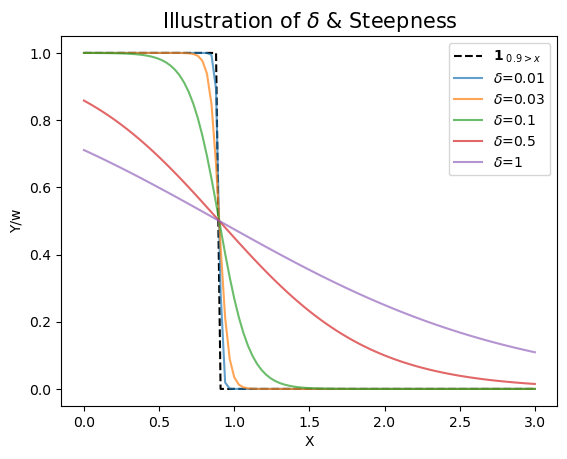
\includegraphics{Illustration_diagrams/SigmoidApprox.png} \emph{Smaller
\(\delta\) leads to closer approximation}

Nonetheless, both the sigmoid approximation and the clamp trick pose
huge challenges to the numeric stability. For the sigmoid function, when
\(\delta\) is too small, there is a great potential for numerical
overflow - the exponents could be tremendous especially when \(X_t\) is
far greater than 0.9, such that \texttt{torch.exp(u)==inf} when
\(u \ge 7.1\). This will raise errors/warnings\footnote{Examples of
  \href{https://discuss.pytorch.org/t/second-order-derivative-with-nan-value-runtimeerror-function-sigmoidbackwardbackward0-returned-nan-values-in-its-0th-output/173260}{RuntimeError}
  and
  \href{https://discuss.pytorch.org/t/output-overflow-and-unstablity-when-use-model-eval/3668}{RuntimeWarning}
  on PyTorch Forums.} in PyTorch. For the clamp trick to work, we must
ensure the initial values strictly fall in \((0,1)\). Thus we propose
\textbf{logit trick} to map the range \([0,1] \to \mathbb{R}\), which
also avoids working with large exponents:

\[
\tilde{Y} := w*\text{logit} (Y/w) = w*\ln\left(\frac{Y/w}{1-Y/w}\right)=f(Y)~.
\]Then apply \(\textit{It}\hat{o} \textit{'s formula}\) (with
superscript \([\cdot]^i\) omiited): \[
\begin{aligned} 
    d \tilde{Y}_t &= (w/2-Y_t)Z_t^2dt + wZ_tdB_t~.\\
\end{aligned}
\]

Correspondingly, we use
\href{https://pytorch.org/docs/stable/generated/torch.nn.BCEWithLogitsLoss.html}{BCEWithLogitsLoss}
as the loss function, which combines a Sigmoid layer and the BCELoss in
one single class. This version is more numerically stable than using a
plain Sigmoid followed by a BCELoss as, by combining the operations into
one layer, it takes advantage of the log-sum-exp trick for numerical
stability.

Worth mentioning, we experimented with multiple combinations of tricks
and loss functions, paired with different optimizers and schedulers.
Eventually we chose
\href{https://pytorch.org/docs/stable/generated/torch.optim.Adamax.html}{Adamax}
and
\href{https://pytorch.org/docs/stable/generated/torch.optim.lr_scheduler.StepLR.html}{StepLR}
due to their relatively better and more stable performance for all cases
in general. Specifically, there are 4 valid combinations of tricks and
loss functions\footnote{Han, J., Long, J. Convergence of the deep BSDE
  method for coupled FBSDEs. Probab Uncertain Quant Risk 5, 5 (2020).}:

\begin{Shaded}
\begin{Highlighting}[]
\NormalTok{\{target\_type: }\StringTok{\textquotesingle{}indicator\textquotesingle{}}\NormalTok{, trick: }\StringTok{\textquotesingle{}logit\textquotesingle{}}\NormalTok{, loss\_type: }\StringTok{\textquotesingle{}BCEWithLogitsLoss\textquotesingle{}}\NormalTok{\}  }\CommentTok{\#\# combo 1}
\NormalTok{\{target\_type: }\StringTok{\textquotesingle{}indicator\textquotesingle{}}\NormalTok{, trick: }\StringTok{\textquotesingle{}clamp\textquotesingle{}}\NormalTok{, loss\_type: }\StringTok{\textquotesingle{}BCELoss\textquotesingle{}}\NormalTok{\}            }\CommentTok{\#\# combo 2}
\NormalTok{\{target\_type: }\StringTok{\textquotesingle{}indicator\textquotesingle{}}\NormalTok{, trick: }\StringTok{\textquotesingle{}clamp\textquotesingle{}}\NormalTok{, loss\_type: }\StringTok{\textquotesingle{}MSELoss\textquotesingle{}}\NormalTok{\}            }\CommentTok{\#\# combo 3}
\NormalTok{\{target\_type: }\StringTok{\textquotesingle{}sigmoid\textquotesingle{}}\NormalTok{  , trick: }\StringTok{\textquotesingle{}clamp\textquotesingle{}}\NormalTok{, loss\_type: }\StringTok{\textquotesingle{}MSELoss\textquotesingle{}}\NormalTok{\}            }\CommentTok{\#\# combo 4}
\end{Highlighting}
\end{Shaded}

:bulb: More details can be found in the
\href{../2Period/Joint_Optim_2Prdx1/README.md}{README} file of
2-agent-2-period scenario.

\hypertarget{results}{%
\subsection{3. Results}\label{results}}

To evaluate and visualize the algorithm performances, we define a
well-wrapped class \texttt{plot\_results}(:bulb:See more details in
\href{../2Period/Joint_Optim_2Prdx1/README.md}{README}), which prodeuces
the following plotted results:

\begin{itemize}
\tightlist
\item
  \textbf{Agents' behaviours and market impacts}

  \begin{itemize}
  \tightlist
  \item
    Learnt optimal control processes
  \item
    Decomposed inventory accumulation pocesses
  \item
    Inventory levels during 2 compliance periods
  \item
    Terminal inventories ready-to-submit
  \item
    Market-clearing prices
  \end{itemize}
\item
  \textbf{Algorithm convergency and learning loss}

  \begin{itemize}
  \tightlist
  \item
    Average forward losses against number of epochs trained
  \item
    Learnt terminal conditions vs.~targtes
  \end{itemize}
\end{itemize}

And here are some example diagramas by algorithms with either
perspectives.

\hypertarget{jointly-optimized-2-agent-2-period}{%
\subsubsection{3.1. Jointly Optimized
2-Agent-2-Period}\label{jointly-optimized-2-agent-2-period}}

\includegraphics{Illustration_Diagrams/joint-2A2P-Sigmoid-ResExamples/Rates.png}
\includegraphics{Illustration_Diagrams/joint-2A2P-Sigmoid-ResExamples/AccumRates.png}
\includegraphics{Illustration_Diagrams/joint-2A2P-Sigmoid-ResExamples/InvAndPrice.png}
\includegraphics{Illustration_Diagrams/joint-2A2P-Sigmoid-ResExamples/InvPreDeli_P1.png}
\includegraphics{Illustration_Diagrams/joint-2A2P-Sigmoid-ResExamples/InvPreDeli_P2.png}
\includegraphics{Illustration_Diagrams/joint-2A2P-Sigmoid-ResExamples/Loss.png}
\includegraphics{Illustration_Diagrams/joint-2A2P-Sigmoid-ResExamples/sigmoid_target.png}

\hypertarget{separately-optimized-2-agent-2-period}{%
\subsubsection{3.2. Separately Optimized
2-Agent-2-Period}\label{separately-optimized-2-agent-2-period}}

\includegraphics{Illustration_Diagrams/Seprt-2A2P-Sigmoid-ResExamples/Rates.png}
\includegraphics{Illustration_Diagrams/Seprt-2A2P-Sigmoid-ResExamples/AccumRates.png}
\includegraphics{Illustration_Diagrams/Seprt-2A2P-Sigmoid-ResExamples/InvAndPrice.png}
\includegraphics{Illustration_Diagrams/Seprt-2A2P-Sigmoid-ResExamples/InvPreDeli_P1.png}
\includegraphics{Illustration_Diagrams/Seprt-2A2P-Sigmoid-ResExamples/InvPreDeli_P2.png}
\includegraphics{Illustration_Diagrams/Seprt-2A2P-Sigmoid-ResExamples/Loss.png}
\includegraphics{Illustration_Diagrams/Seprt-2A2P-Sigmoid-ResExamples/sigmoid_target.png}

\hypertarget{comparisons-and-analyses}{%
\subsubsection{3.3. Comparisons And
Analyses}\label{comparisons-and-analyses}}

\hypertarget{joint-vs-separate-optimization}{%
\paragraph{3.3.1. Joint Vs Separate
Optimization}\label{joint-vs-separate-optimization}}

Upon comparing the shown results from 2 different perspectives, one can
get very instructive and enlighting implications.

By planning ahead in the \textbf{first period} out of a long-term view,
agents tend to invest more in expansion even at the end of the first
period, whereas when only dedicated to meeting the current target, all
agents reduce the expansion rate to zero since there's no point
investing in delayed payoffs. Similarly, the short-sighted agents will
trade more actively and might work more overtime at the first period end
in sought of immediate paybacks. Consequently, almost of these agents
unawaring of the upcoming second compliance period will end up ``just''
meet the quota of 0.9 at \(T_1\), since any extra inventory would be
regarded ``useless'' - yet find themselves having to start over from
almost scratch in order to meet the second quota. This can be seen from
the first columns of inventory histograms and the inventory level plots.

Therefore in the \textbf{second period}, agents starting from 0
inventory will either try very hard to make up for expansion
(examplified by the green ``pop1''), or rely heavily on overhours and
trading (examplified by the red ``pop2''), which pushes the market price
even higher in the second period. However, both populations would
ultimately realize the quota is almost impossible to meet and give up at
all. This is shown by a great proportion of \(Y_{T_2}^i=w\). Contrarily,
only until the true ``end of the world'' (i.e.~\(T_2\)) approaches,
those who have maintained a reasonable level of stocks start to
gradually reduce expansion and sell any extra inventories. And since
most of them have already accumulated a relatively high baseline rate,
there's less need for them to work overtime or purchase inventories than
in the first period (shown by the decreased slopes of the accumulated
generation plots) - thus the market price goes down.

\hypertarget{sub-population-1-vs-2}{%
\paragraph{3.3.2. Sub-Population 1 Vs 2}\label{sub-population-1-vs-2}}

Then let's take a closer look at either case, analizing the differences
made by distinctive preferences and initial conditions across
sub-populations. Starting at generally lower initial level (\(v^1>v^2\))
yet blessed with greater baseline rate (\(h^1<h^2\)), ``pop2'' wouldn't
worry as much as the green guys ``pop1'' in terms of expansion, and find
working overtime or trading more rewarding. Even further, the red guys
would be more interested in overtimes than in trading since it's
``cheaper'' per unit inventory, which is the opposite for the green guys
(i.e.~\(\zeta^1>\gamma^1, \zeta^2<\gamma^2\)).

However, regardless of agents' perspectives (long/short-term), the
explicit initial advantage in inventory level and the implicit
disavantage in baseline capacity makes the green guys ``lazier'',
i.e.~less motivated to working extra-hours. Consequently, in the second
complience period, they are more likely to find themselves hard pressed
to meet the quota and have to purchase from the red guys, which is
indicated by the trends and signs (positive for buying and vice versa)
of accumulated trading amount.

\hypertarget{model-performance}{%
\paragraph{3.3.3. Model Performance}\label{model-performance}}

And both algorithms produce descending loss plots and learnt terminal
conditions that almost overlapping with their targets (black dots) given
\(X_{T_1}^i, X_{T_2}^i\), which suggests desiredly converging and stable
of model performance. Worth mentioning, since \emph{sigmoid targets}
with \emph{MSELoss} have greatest differentibility, combined with small
\(w\) (e.g.~0.25) narrowing down the step from 0 to \(w\), models set up
as such would produce rather good-looking results. Certainly, there
might be other parameter and model settings leading to greater
convergence and stability, which are open for experimenting.

\hypertarget{conclusions-and-takeaways}{%
\section{4. Conclusions And Takeaways}\label{conclusions-and-takeaways}}

From the results and analysis above, one can take away some instructive
implications and apply not only to the REC markets, but also in her/his
daily life.

\begin{quote}
\begin{itemize}
\tightlist
\item
  Always plan ahead and condiser for the future.
\item
  Always do slightly more than required and maintain a reasonable level
  of backups.
\item
  Don't be blinded by the apparent advatages/achievements, instead care
  for the growth rate and capacity - that's what you can carry to the
  future for sure.
\item
  When the majority gets lazy for short-sighted, the market gets worse -
  where any individual will be affected more or less.
\end{itemize}
\end{quote}

\begin{center}\rule{0.5\linewidth}{0.5pt}\end{center}

\hypertarget{references}{%
\section{References:}\label{references}}

\href{https://doi.org/10.48550/arXiv.2110.01127}{{[}1{]}}
\href{https://arxiv.org/abs/1210.5780}{{[}2{]}}

\end{document}
